\documentclass[12pt,a4paper]{article}
\usepackage{cmap} % Makes the PDF copiable. See http://tex.stackexchange.com/a/64198/25761
\usepackage[T1]{fontenc}
\usepackage[brazil]{babel}
\usepackage[utf8]{inputenc}
\usepackage{amsmath}
\usepackage{amsfonts}
\usepackage{amssymb}
\usepackage{amsthm}
\usepackage[usenames,svgnames,dvipsnames]{xcolor}
\usepackage{hyperref}
\usepackage{multicol}
\usepackage{graphicx}
\usepackage[margin=2cm]{geometry}

\hypersetup{
    colorlinks = true,
    allcolors = {blue}
}

% TODO: Consider using exsheets
% http://linorg.usp.br/CTAN/macros/latex/contrib/exsheets/exsheets_en.pdf
%
% http://ctan.org/tex-archive/macros/latex/contrib/exercise/
% Options: answerdelayed,lastexercise,noanswer
\usepackage[answerdelayed,lastexercise]{exercise}

\addto\captionsbrazil{%
\def\listexercisename{Lista de exerc\'icios}%
\def\ExerciseName{Exerc\'icio}%
\def\AnswerName{Solu\c{c}\~ao do exerc\'icio}%
\def\ExerciseListName{Ex.}%
\def\AnswerListName{Solu\c{c}\~ao}%
\def\ExePartName{Parte}%
\def\ArticleOf{de\ }%
}

\renewcommand{\ExerciseHeaderTitle}{(\ExerciseTitle)\ }
\renewcommand{\ExerciseListHeader}{%\ExerciseHeaderDifficulty%
\textbf{%\ExerciseListName\
\ExerciseHeaderNB.\ %
%\ --- \
\ExerciseHeaderTitle}%
%\ExerciseHeaderOrigin
\ignorespaces}
\renewcommand{\AnswerListHeader}{\textbf{\ExerciseHeaderNB.\ (\AnswerListName)\ }}

\newtheorem*{note}{Observação}
\newcommand{\fixme}{{\color{red}(...)}}
\newcommand*\diff{\mathop{}\!\mathrm{d}}
\newcommand*\sen{\operatorname{sen}}
\newcommand*\tg{\operatorname{tg}}
\newcommand*\cotg{\operatorname{cotg}}
\newcommand*\cosec{\operatorname{cossec}}
\newcommand*\cotgh{\operatorname{cotgh}}
\newcommand*\arcsen{\operatorname{arcsen}}
\newcommand*\arctg{\operatorname{arctg}}
\newcommand*\abs[1]{\left|#1\right|}
\newcommand*\R{\mathbb{R}}
\newcommand*\op[1]{\overset{#1}{\rightarrow}}

\renewcommand{\theenumi}{\alph{enumi}}
\renewcommand\labelenumi{(\theenumi) }

\newcommand*\tipo{Prova I}
\newcommand*\turma{PRO112-02U}
\newcommand*\disciplina{CDI2001}
\newcommand*\eu{Helder G. G. de Lima}
\newcommand*\data{13/09/2024}

\author{\eu}
\title{\tipo - \disciplina}
\date{\data}

\begin{document}
\thispagestyle{empty}
\newgeometry{margin=2cm,bottom=0.5cm}
\begin{center}

\includegraphics[width=9.0cm]{marca} \\
\textbf{\tipo\ (\disciplina / \turma)} \\
Prof. \eu\footnote{
Este é um material de acesso livre distribuído sob os termos da licença \href{https://creativecommons.org/licenses/by-sa/4.0/deed.pt_BR}{Creative Commons BY-SA 4.0}}
\end{center}

\noindent Nome do(a) aluno(a): \underline{\hspace{9,7cm}} Data: \underline{\data}

\begin{center}\fbox{
\begin{minipage}{14cm}

{\footnotesize
\begin{itemize}
\renewcommand{\theenumi}{\Roman{enumi}}
\item Identifique-se em todas as folhas.
\item Mantenha o celular e os demais equipamentos eletrônicos desligados durante a prova.
\item Justifique cada resposta com cálculos ou argumentos baseados na teoria estudada.
\item Resolva $4$ das $5$ questões (deixe claro que questão não deverá ser corrigida).
\end{itemize}
}

\end{minipage}
}
\end{center}

\begin{ExerciseList}
\Exercise[title={2,5}] Calcule a área da região delimitada pelas curvas $y=2\cos(x)$ e $y=2\cos(2x)$, no intervalo $-\frac{2\pi}{3}\leq x\leq \frac{2\pi}{3}$.
\Answer Para todo $x \in [-\frac{2\pi}{3}, \frac{2\pi}{3}]$, tem-se $2\cos(2x) \leq 2\cos(x)$, como pode ser observado na figura a seguir:

\begin{center}
  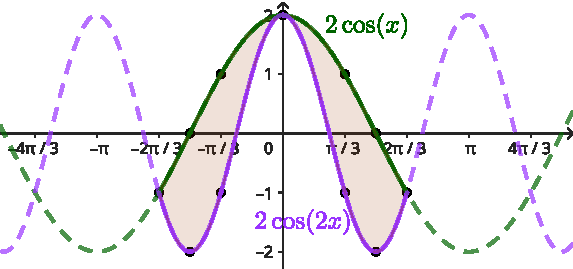
\includegraphics[height=4cm]{img/região-entre-trigonométricas.pdf}
\end{center}

Considerando que as funções dadas são pares, a área da região especificada é dada pela integral:
\begin{align*}
  A
  & = \int_{-\frac{2\pi}{3}}^{\frac{2\pi}{3}} 2\cos(x) -2\cos(2x)\diff{x}
    = 2\int_{0}^{\frac{2\pi}{3}} 2\cos(x) -2\cos(2x)\diff{x}
    = 2 \left[2\sen(x) - \sen(2x)\right]_{0}^{\frac{2\pi}{3}} \\
    & = 2 \left[2\sen\left(\frac{2\pi}{3}\right) - \sen\left(\frac{4\pi}{3}\right) - (0 - 0)\right]
    = 2 \left[2\frac{\sqrt{3}}{2} - \left(-\frac{\sqrt{3}}{2}\right)\right]
    = \boxed{3 \sqrt{3} \text{ u.a.}}.
\end{align*}

\Exercise[title={2,5}] Calcule, caso seja convergente, a integral imprópria $\int_{0}^\infty \frac{12}{x^2+4} \diff{x}$.
\Answer Como o intervalo de integração não é finito, tem-se:
\[
  \int_{0}^\infty \frac{12}{x^2+4} \diff{x}
  = \lim_{t\to \infty} \int_0^t \frac{12}{x^2+4} \diff{x}.
\]
Fazendo a mudança de variável $x=2\tan(\theta)$, tem-se $\diff{x} = 2\sec^2(\theta)\diff{\theta}$. Além disso, para $x=t$, tem-se $\theta = \arctan(t/2)$ e para $x=0$ tem-se $\theta=0$, então:
\begin{align*}
  \int_{0}^\infty \frac{12}{x^2+4} \diff{x}
  & = \lim_{t\to \infty} \int_0^{\arctan(t/2)} \frac{12}{2\sec^2(\theta)} 2\sec^2(\theta)\diff{\theta}
  = \lim_{t\to \infty} \int_0^{\arctan(t/2)} 6 \diff{\theta} \\
  & = \lim_{t\to \infty} (6\theta)\bigg|_{0}^{\arctan(t/2)}
  = \lim_{t\to \infty} 6\arctan\left(\frac{t}{2}\right) - 0
  = 6\cdot \frac{\pi}{2}
  = \boxed{3\pi}.
\end{align*}

\begin{center}
  \includegraphics[height=4cm]{img/integral-imprópria.pdf}
\end{center}



\Exercise[title={2,5}] Calcule a área da região indicada, que é interior à circunferência \(r = 1\), está acima do eixo polar e à direita da primeira pétala da rosácea \(r = \sen(2\theta)\):

\begin{center}
  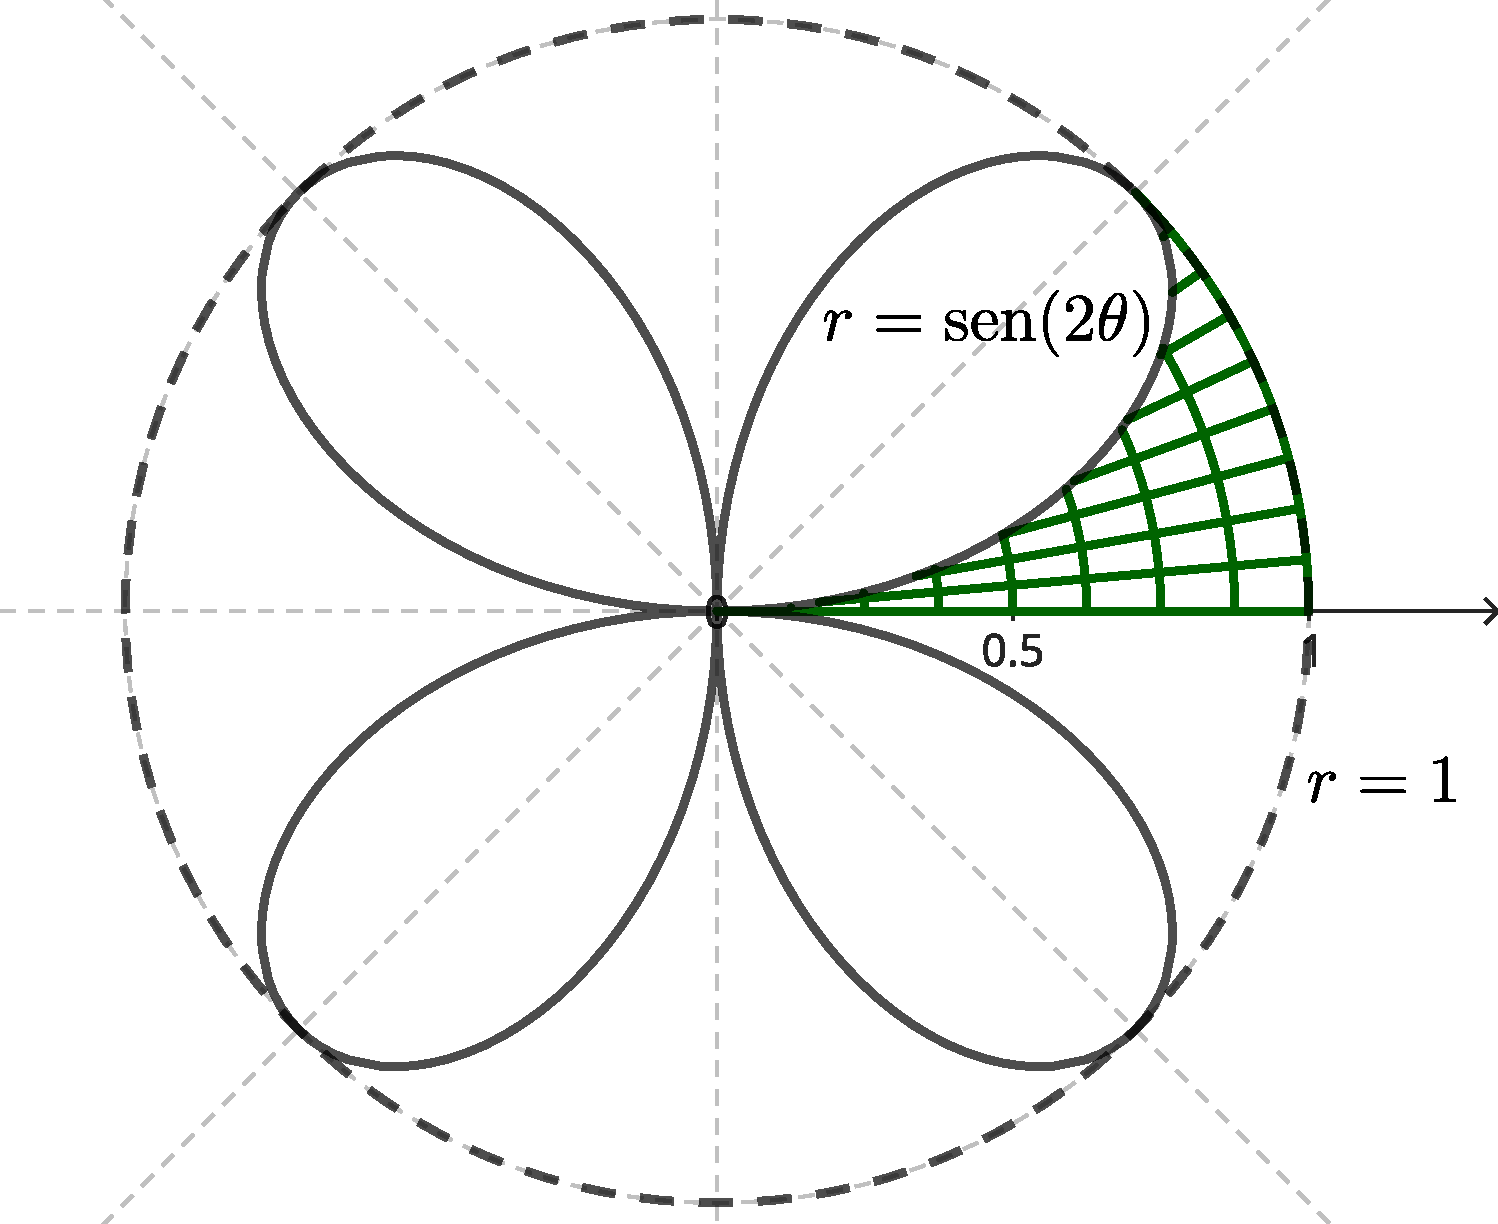
\includegraphics[width=6.0cm]{img/curvas-polares.pdf}
\end{center}

\Answer \textbf{Solução 1}: Primeiro, determinamos o ângulo da interseção entre a circunferência \(r = 1\) e a rosácea \(r = \sen(2\theta)\). Igualando as equações das duas curvas:

\[
1 = \sen(2\theta),
\]

temos que \(\sen(2\theta) = 1\), o que ocorre quando \(2\theta = \frac{\pi}{2}\), ou seja, \(\theta = \frac{\pi}{4}\).

Agora, a área da região hachurada é obtida subtraindo a área da parte da rosácea \(r = \sen(2\theta)\) da área do setor circular de raio \(r = 1\) e ângulo \(\theta = \frac{\pi}{4}\). Assim, a área \(A\) da região é dada por:

\[
A
= \frac{1}{2}\int_0^{\pi/4} 1^2 \diff\theta - \frac{1}{2}\int_0^{\pi/4} \left(\sen(2\theta)\right)^2 \diff\theta
= \frac{1}{2} \int_0^{\pi/4} \left[1 - \left(\sen(2\theta)\right)^2 \right] \diff\theta.
\]

Utilizando a identidade trigonométrica \(\sen^2(2\theta) = \frac{1}{2}\left(1 - \cos(4\theta)\right)\):

\[
A = \frac{1}{2} \int_0^{\pi/4} \left[1 - \frac{1}{2}\left(1 - \cos(4\theta)\right)\right] \diff\theta = \frac{1}{2} \int_0^{\pi/4} \left[\frac{1}{2} + \frac{1}{2}\cos(4\theta)\right] \diff\theta.
\]

Aplicando o teorema fundamental do cálculo:

\begin{align*}
A
& = \frac{1}{4} \int_0^{\pi/4} \left[1 + \cos(4\theta)\right] \diff\theta
= \frac{1}{4} \left(\theta + \frac{\sen(4\theta)}{4}\right)\bigg|_0^{\pi/4} \\
& = \frac{1}{4} \left(\frac{\pi}{4} + \frac{0}{4} - (0 + 0)\right)
= \boxed{\frac{\pi}{16} \text{ u.a.}}.
\end{align*}

\textbf{Solução 2}: Devido à simetria da rosácea e da circunferência em relação à reta $\theta = \frac{\pi}{4}$, obteríamos o mesmo resultado se considerássemos $0 \leq \theta \leq \frac{\pi}{2}$ e dividíssemos a área obtida por dois.


\Exercise[title={2,5}] Determine o comprimento de arco de $y=x^{3/2}$, entre $x=0$ e $x=1$.
\Answer A fórmula para o comprimento de arco é dada por:
\[
  L = \int_a^b \sqrt{1 + [f'(x)]^2} \, dx
\]
Considerando que $y^\prime = \frac{3}{2}x^{1/2} = \frac{3}{2}\sqrt{x}$, tem-se:
\[
  L
  = \int_0^1 \sqrt{1 + \left(\frac{3}{2}\sqrt{x}\right)^2} \diff{x}
  = \int_0^1 \sqrt{1 + \frac{9}{4}x} \diff{x}
\]

Fazendo a mudança de variáveis $u=1 + \frac{9}{4}x$, tem-se $x=\frac{4}{9}(u-1)$ e $\diff{x} = \frac{4}{9}\diff{u}$. Assim, os limites de integração mudam para $u=1$ e $u=\frac{13}{4}$:
\[
  L = \int_1^{13/4} \frac{4}{9}\sqrt{u} \diff{u}
  = \frac{4}{9}\cdot\frac{2}{3}u^{ \frac{3}{2}}\bigg|_1^{13/4}
  = \frac{8}{27}u^{ \frac{3}{2}}\bigg|_1^{13/4}
  = \frac{8}{27} \left(\frac{13}{4}\right)^{3/2} - \frac{8}{27}
  = \boxed{\frac{13\sqrt{13}}{27} - \frac{8}{27} \text{ u.a.}}
\]

\Exercise[title={2,5}] Calcule o volume do sólido gerado pela rotação, em torno do eixo $x$, da região delimitada pelo gráfico da função $f(x) = 2\sqrt{x} e^x$, e pelas retas verticais $x=0$ e $x=1$.
\Answer O sólido de revolução é mostrado na figura a seguir:
\begin{center}
  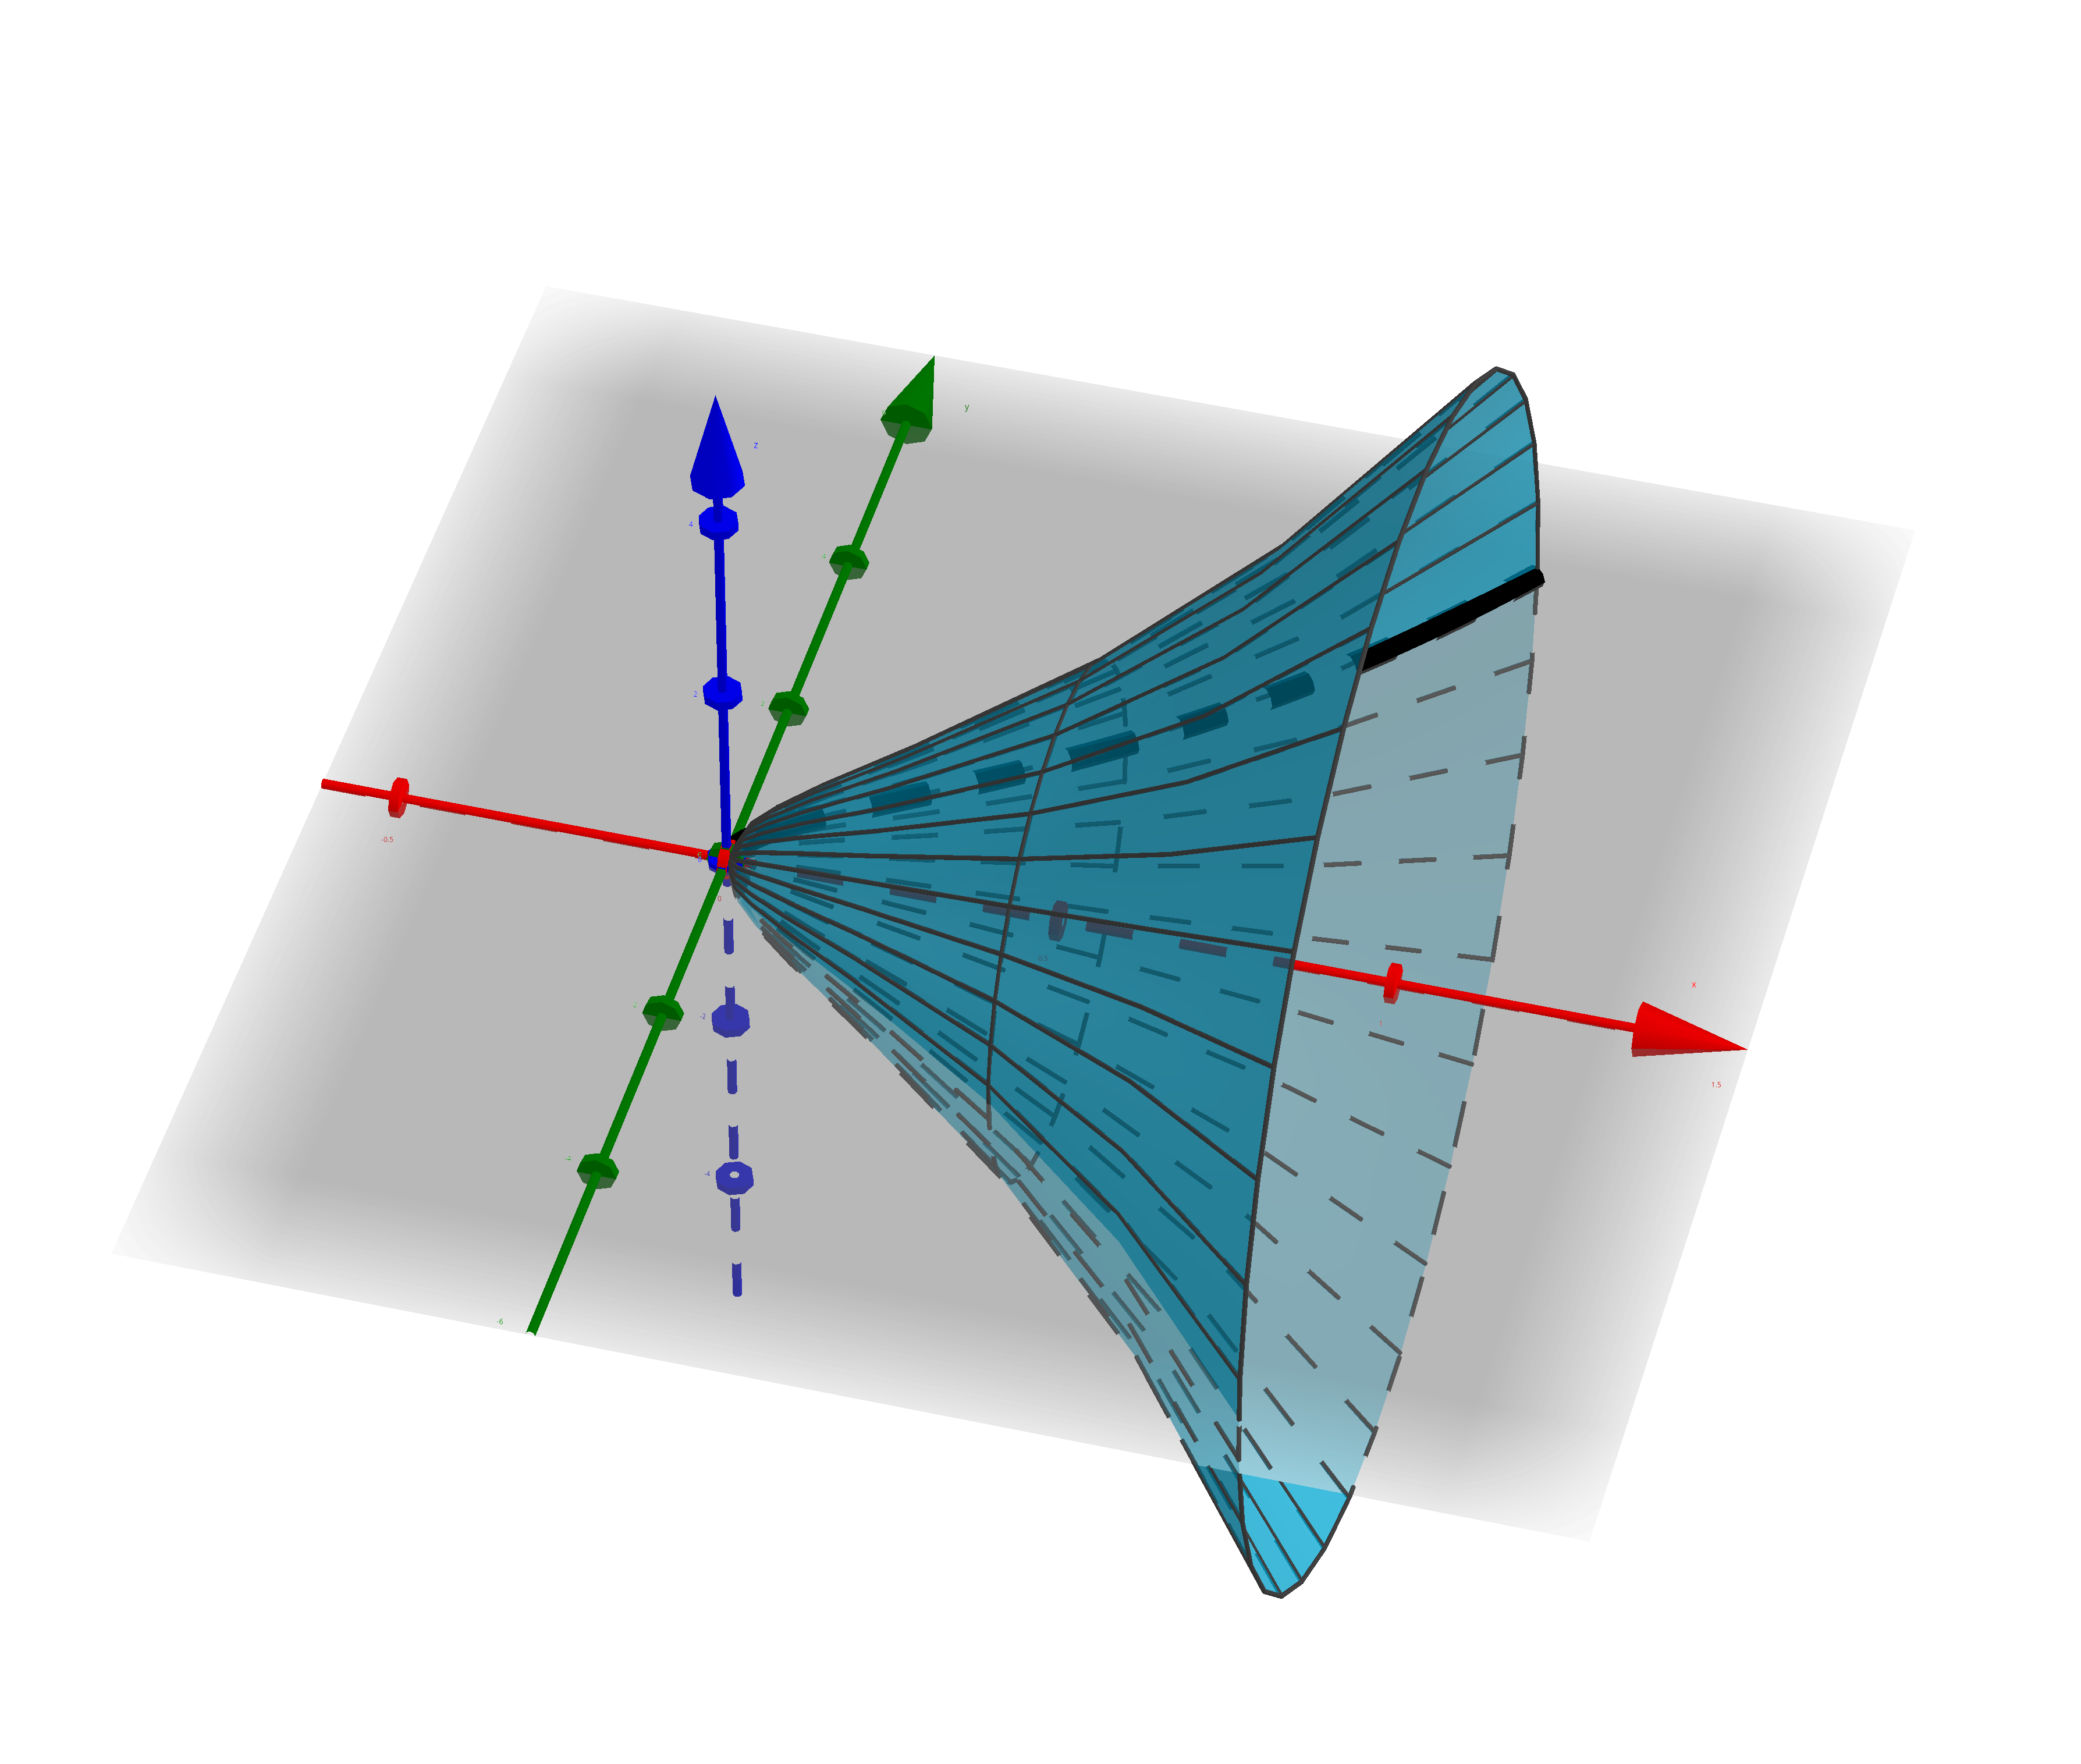
\includegraphics[height=6.6cm]{img/sólido-de-revolução.png}
\end{center}

O volume do sólido é dado pela integral da área das seções transversais. Como as seções transversais são discos com raio $f(x)$, o volume é:

\[
V = \int_0^1 \pi \left[2\sqrt{x}e^x\right]^2 \diff{x} = \int_0^1 4\pi x e^{2x} \diff{x} = 2\pi \int_0^1 x \cdot 2e^{2x} \diff{x}.
\]

Usando integração por partes, com \(u = x\) e \(\diff{v} = 2e^{2x}\), temos \(\diff{u} = \diff{x}\) e \(v = e^{2x}\). Portanto,

\begin{align*}
V
& = 2\pi \left[\left(x e^{2x} \right)\big|_0^1  - \int_0^1 e^{2x} \diff{x}\right]
= 2\pi \left[ (e^{2} - 0) - \left(\frac{e^{2x}}{2} \right)\bigg|_0^1\right]
= 2\pi \left[ e^{2} - \left(\frac{e^{2}}{2} - \frac{1}{2} \right)\right] \\
& =2\pi \left[ \frac{e^{2}}{2} + \frac{1}{2}\right]
= \pi e^{2} + \pi
= \boxed{\pi \left( e^2 + 1 \right) \text{ u.v.}}.
\end{align*}
\end{ExerciseList}

\vfill
\begin{center}
BOA PROVA!
\end{center}

\newpage
\restoregeometry
\section*{Respostas}
\shipoutAnswer
\end{document}
